\chapter{Game Theory}

\section{Introduction}

In this chapter, we introduce the most important methodology in modern economics: \textbf{Game Theory}. This represents a meaningful digression from the standard themes of microeconomics, serving to sharpen our analytical tools.

Game theory models \textbf{strategic behavior} by agents who understand that their actions affect the actions of other agents. But what do we mean by strategic behavior?
\begin{itemize}
    \item Rational behavior in the context of a small number of agents.
    \item Examples include two firms in a duopoly market, or two players playing Chinese Chess or Weiqi.
\end{itemize}

\begin{definition}[Game]
    A game consists of:
    \begin{enumerate}
        \item A set of \textbf{players}.
        \item A set of \textbf{strategies} for each player.
        \item The \textbf{payoffs} to each player for every possible list of strategy choices by the players.
    \end{enumerate}
\end{definition}

In this course, we will focus primarily on \textbf{Two-Player Games}, where each player can choose between only two strategies.

\section{Simultaneous-Move Games and Nash Equilibrium}

\subsection{Payoff Matrix}

Consider a game with two players, Player A and Player B.
\begin{itemize}
    \item Player A has two strategies: "Up" ($U$) and "Down" ($D$).
    \item Player B has two strategies: "Left" ($L$) and "Right" ($R$).
\end{itemize}

We represent the payoffs in a \textbf{payoff matrix}. The first number in each cell is Player A's payoff, and the second is Player B's payoff.

\begin{table}[h]
    \centering
    \renewcommand{\arraystretch}{1.5}
    \begin{tabular}{cc|c|c|}
      & \multicolumn{1}{c}{} & \multicolumn{2}{c}{\textbf{Player B}} \\
      & \multicolumn{1}{c}{} & \multicolumn{1}{c}{$L$}  & \multicolumn{1}{c}{$R$} \\ \cline{3-4}
      \multirow{2}*{\textbf{Player A}}  & $U$ & $(3,9)$ & $(1,8)$ \\ \cline{3-4}
      & $D$ & $(0,0)$ & $(2,1)$ \\ \cline{3-4}
    \end{tabular}
    \caption{A Payoff Matrix Example}
    \label{tab:game_matrix_1}
\end{table}

A \textbf{play} of the game is a pair, such as $(U,R)$, where the first element is the strategy chosen by Player A and the second is the strategy chosen by Player B.

\subsection{Determining the Outcome}

To analyze which plays are likely, we look at \textbf{Best Responses}:
\begin{itemize}
    \item If Player B plays \textit{Right}: Player A compares playing $U$ (payoff 1) vs $D$ (payoff 2). Since $2 > 1$, A's best reply is $D$. Thus, $(U,R)$ is unlikely.
    \item If Player A plays \textit{Down}: Player B compares playing $L$ (payoff 0) vs $R$ (payoff 1). Since $1 > 0$, B's best reply is $R$.
    \item If Player A plays \textit{Up}: Player B compares playing $L$ (payoff 9) vs $R$ (payoff 8). Since $9 > 8$, B's best reply is $L$.
\end{itemize}

\begin{definition}[Nash Equilibrium]
    A play of the game where each strategy is a \textbf{best reply} to the other is a \textbf{Nash Equilibrium} (NE).
\end{definition}

In the example above (Table \ref{tab:game_matrix_1}), we can identify the Nash Equilibria by checking for mutual best responses:
\begin{itemize}
    \item $(U,L)$: If A plays $U$, B prefers $L$ ($9>8$). If B plays $L$, A prefers $U$ ($3>0$). \textbf{This is a Nash Equilibrium.}
    \item $(D,R)$: If A plays $D$, B prefers $R$ ($1>0$). If B plays $R$, A prefers $D$ ($2>1$). \textbf{This is also a Nash Equilibrium.}
\end{itemize}
Notice that $(U,L)$ is preferred to $(D,R)$ by both players (payoffs $3,9$ vs $2,1$), but both are stable outcomes.

\section{The Prisoner's Dilemma}

To see if Pareto-preferred outcomes must be what we see in the play of a game, consider the famous \textbf{Prisoner's Dilemma}.

\begin{examplebox}{The Prisoner's Dilemma}
    Two prisoners, Bonnie and Clyde, have two strategies: Silence ($S$) or Confess ($C$).
    
    \begin{center}
    \renewcommand{\arraystretch}{1.5}
    \begin{tabular}{cc|c|c|}
      & \multicolumn{1}{c}{} & \multicolumn{2}{c}{\textbf{Clyde}} \\
      & \multicolumn{1}{c}{} & \multicolumn{1}{c}{$S$}  & \multicolumn{1}{c}{$C$} \\ \cline{3-4}
      \multirow{2}*{\textbf{Bonnie}}  & $S$ & $(-5,-5)$ & $(-30,-1)$ \\ \cline{3-4}
      & $C$ & $(-1,-30)$ & $(-10,-10)$ \\ \cline{3-4}
    \end{tabular}
    \end{center}

    \textbf{Analysis:}
    \begin{itemize}
        \item \textbf{For Clyde:} 
        If Bonnie plays $S$, Clyde prefers $C$ ($-1 > -5$). 
        If Bonnie plays $C$, Clyde prefers $C$ ($-10 > -30$).
        Regardless of Bonnie's choice, Clyde's best reply is always Confess.
        \item \textbf{For Bonnie:} Similarly, no matter what Clyde plays, Bonnie's best reply is always Confess.
    \end{itemize}
    
    Strategy $C$ is a \textbf{Dominant Strategy} for both players.
    
    \textbf{Result:} The only Nash equilibrium is $(C,C)$ with payoffs $(-10, -10)$. However, outcome $(S,S)$ with payoffs $(-5, -5)$ would be better for both. Thus, the only Nash equilibrium is \textbf{inefficient}.
\end{examplebox}

\section{Sequential Games}

So far, we have discussed \textbf{simultaneous play games}, where players choose strategies at the same time. In \textbf{sequential play games}, one player plays before another.
\begin{itemize}
    \item The player who plays first is the \textbf{Leader}.
    \item The player who plays second is the \textbf{Follower}.
\end{itemize}

Recall our first example (Table \ref{tab:game_matrix_1}) which had two Nash equilibria: $(U,L)$ and $(D,R)$. In a simultaneous game, it is hard to say which occurs. However, structure changes if the game is sequential.

\subsection{Extensive Form (Game Tree)}

Suppose Player A moves first. We can represent this using a game tree (Extensive Form).

\begin{center}
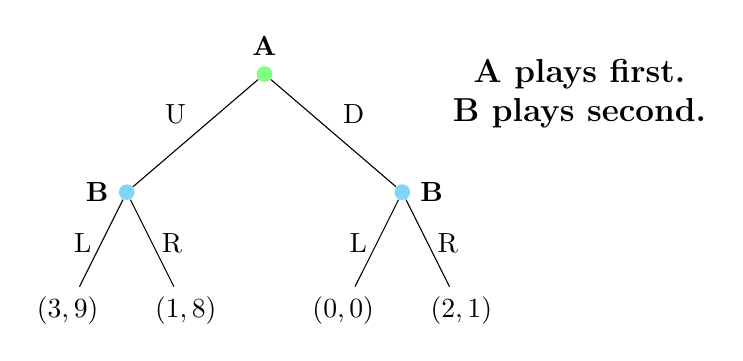
\begin{tikzpicture}[level distance=1.5cm,
  level 1/.style={sibling distance=3.5cm},
  level 2/.style={sibling distance=1.5cm}]
  \node[circle, fill=green!50, inner sep=2pt, label=above:\textbf{A}] {}
    child {node[circle, fill=cyan!50, inner sep=2pt, label=left:\textbf{B}] {}
      child {node {$(3,9)$} edge from parent node[left] {L}}
      child {node {$(1,8)$} edge from parent node[right] {R}}
      edge from parent node[above left] {U}
    }
    child {node[circle, fill=cyan!50, inner sep=2pt, label=right:\textbf{B}] {}
      child {node {$(0,0)$} edge from parent node[left] {L}}
      child {node {$(2,1)$} edge from parent node[right] {R}}
      edge from parent node[above right] {D}
    };
    \node at (4,0) {\large \textbf{A plays first.}};
    \node at (4,-0.5) {\large \textbf{B plays second.}};
\end{tikzpicture}
\end{center}

\subsection{Backward Induction}
To solve this, we reason backwards:
\begin{enumerate}
    \item \textbf{B's decision:}
    \begin{itemize}
        \item If A plays $U$, B chooses between $L$ (9) and $R$ (8). B chooses $L$. Payoff to A is 3.
        \item If A plays $D$, B chooses between $L$ (0) and $R$ (1). B chooses $R$. Payoff to A is 2.
    \end{itemize}
    \item \textbf{A's decision:} A knows B's optimal responses. A effectively chooses between the outcome of playing $U$ (which leads to $L$, giving A 3) and playing $D$ (which leads to $R$, giving A 2).
    \item Since $3 > 2$, A plays $U$.
\end{enumerate}

Thus, in the sequential version, $(U,L)$ is the likely Nash equilibrium.

\section{Mixed Strategies}

\subsection{Pure vs. Mixed Strategies}
Strategies like "Up", "Down", "Left", or "Right" are called \textbf{Pure Strategies}. Some games have no Nash equilibrium in pure strategies.

\begin{examplebox}{Matching Pennies / Competitive Game}
    Consider the following game:
    \begin{center}
    \renewcommand{\arraystretch}{1.5}
    \begin{tabular}{cc|c|c|}
      & \multicolumn{1}{c}{} & \multicolumn{2}{c}{\textbf{Player B}} \\
      & \multicolumn{1}{c}{} & \multicolumn{1}{c}{$L$}  & \multicolumn{1}{c}{$R$} \\ \cline{3-4}
      \multirow{2}*{\textbf{Player A}}  & $U$ & $(1,2)$ & $(0,4)$ \\ \cline{3-4}
      & $D$ & $(0,5)$ & $(3,2)$ \\ \cline{3-4}
    \end{tabular}
    \end{center}
    \textbf{Check for Pure NE:}
    \begin{itemize}
        \item $(U,L)$: B prefers $R$ ($4>2$). Not NE.
        \item $(U,R)$: A prefers $D$ ($3>0$). Not NE.
        \item $(D,R)$: B prefers $L$ ($5>2$). Not NE.
        \item $(D,L)$: A prefers $U$ ($1>0$). Not NE.
    \end{itemize}
    This game has \textbf{no pure strategy Nash equilibria}.
\end{examplebox}

However, a Nash equilibrium always exists if we allow for \textbf{Mixed Strategies}.
\begin{definition}[Mixed Strategy]
    A mixed strategy involves selecting a probability distribution over pure strategies.
    \begin{itemize}
        \item Player A plays $U$ with probability $\pi_U$ (or $p$) and $D$ with probability $1-\pi_U$.
        \item Player B plays $L$ with probability $\pi_L$ (or $q$) and $R$ with probability $1-\pi_L$.
    \end{itemize}
\end{definition}

\subsection{Calculating Mixed Strategy Equilibrium}

Let's compute the equilibrium for a standard example where pure strategies exist but we want to see the general method, or for games like the one above where only mixed strategies exist. Consider this generic payoff matrix:

\begin{center}
\renewcommand{\arraystretch}{1.5}
\begin{tabular}{cc|c|c|}
  & \multicolumn{1}{c}{} & \multicolumn{2}{c}{\textbf{Player B}} \\
  & \multicolumn{1}{c}{} & \multicolumn{1}{c}{$L$ ($q$)}  & \multicolumn{1}{c}{$R$ ($1-q$)} \\ \cline{3-4}
  \multirow{2}*{\textbf{Player A}}  & $U$ ($p$) & $(6,4)$ & $(3,5)$ \\ \cline{3-4}
  & $D$ ($1-p$) & $(4,3)$ & $(5,7)$ \\ \cline{3-4}
\end{tabular}
\end{center}

\subsubsection{Player A's Best Response}
We calculate Player A's \textbf{Expected Value (EV)} for playing purely $U$ or purely $D$, given B plays $L$ with probability $q$.
\begin{align*}
    EV^A(U) &= 6q + 3(1-q) = 3 + 3q \\
    EV^A(D) &= 4q + 5(1-q) = 5 - q
\end{align*}
Player A will choose $U$ if $EV^A(U) > EV^A(D)$:
\begin{align*}
    3 + 3q &> 5 - q \\
    4q &> 2 \implies q > 1/2
\end{align*}
Thus, A's best response strategy ($p$) is:
\begin{itemize}
    \item If $q > 1/2$, play $U$ ($p=1$).
    \item If $q < 1/2$, play $D$ ($p=0$).
    \item If $q = 1/2$, A is indifferent ($0 \le p \le 1$).
\end{itemize}

\subsubsection{Player B's Best Response}
Similarly, we calculate B's EV given A plays $U$ with probability $p$.
\begin{align*}
    EV^B(L) &= 4p + 3(1-p) = 3 + p \\
    EV^B(R) &= 5p + 7(1-p) = 7 - 2p
\end{align*}
Player B plays $L$ if $EV^B(L) > EV^B(R)$:
\begin{align*}
    3 + p &> 7 - 2p \\
    3p &> 4 \implies p > 4/3
\end{align*}
Since $p$ is a probability, it cannot exceed 1. Therefore, $3+p$ is \textbf{always less than} $7-2p$ (for valid range $0 \le p \le 1$). 
\begin{itemize}
    \item B's best response is always to play $R$ ($q=0$). $R$ is a strictly dominant strategy for B in this numerical example.
\end{itemize}

\subsubsection{Finding the Nash Equilibrium}
The Nash Equilibrium is the intersection of the best response curves.
\begin{itemize}
    \item A wants to match $q$.
    \item B always plays $q=0$.
    \item If $q=0$, A's best response is $D$ (since $q < 1/2$).
    \item Result: Pure strategy equilibrium $(D, R)$.
\end{itemize}

\subsection{Case with Multiple Equilibria (Hawk-Dove Game)}

Let's analyze a game of coexistence where mixed strategies are essential.
\begin{examplebox}{Hawk-Dove Game}
    Two animals (e.g., bears) contest a resource. They can be a \textbf{Hawk} (Aggressive) or a \textbf{Dove} (Passive).
    
    \begin{center}
    \renewcommand{\arraystretch}{1.5}
    \begin{tabular}{cc|c|c|}
      & \multicolumn{1}{c}{} & \multicolumn{2}{c}{\textbf{Bear 2}} \\
      & \multicolumn{1}{c}{} & \multicolumn{1}{c}{$H$ ($\pi_H^2$)}  & \multicolumn{1}{c}{$D$} \\ \cline{3-4}
      \multirow{2}*{\textbf{Bear 1}}  & $H$ ($\pi_H^1$) & $(-5,-5)$ & $(8,0)$ \\ \cline{3-4}
      & $D$ & $(0,8)$ & $(4,4)$ \\ \cline{3-4}
    \end{tabular}
    \end{center}
    
    \textbf{Pure Strategy Equilibria:}
    \begin{itemize}
        \item $(H,D)$ is a NE ($8>4$ for Bear 1, $0>-5$ for Bear 2).
        \item $(D,H)$ is a NE ($0>-5$ for Bear 1, $8>4$ for Bear 2).
        \item Note: $(D,D)$ is not a NE because a Hawk beats a Dove ($8>4$). $(H,H)$ is not a NE because fighting hurts both ($-5 < 0$).
    \end{itemize}
\end{examplebox}

\textbf{Mixed Strategy Equilibrium Calculation:}
Let $\pi_H^1$ be prob. Bear 1 is Hawk, $\pi_H^2$ be prob. Bear 2 is Hawk.

For Bear 1 to mix strategies, it must be indifferent between H and D:
\begin{align*}
    EV^1(H) &= -5\pi_H^2 + 8(1-\pi_H^2) = 8 - 13\pi_H^2 \\
    EV^1(D) &= 0\pi_H^2 + 4(1-\pi_H^2) = 4 - 4\pi_H^2
\end{align*}
Set $EV^1(H) = EV^1(D)$:
\begin{align*}
    8 - 13\pi_H^2 &= 4 - 4\pi_H^2 \\
    4 &= 9\pi_H^2 \\
    \pi_H^2 &= 4/9
\end{align*}
By symmetry, Bear 2 is indifferent when $\pi_H^1 = 4/9$.

\textbf{Best Response Dynamics:}
\begin{itemize}
    \item Bear 1 plays $H$ if $\pi_H^2 < 4/9$.
    \item Bear 1 plays $D$ if $\pi_H^2 > 4/9$.
\end{itemize}

This creates a reaction function plot where the two curves intersect at $(\pi_H^1, \pi_H^2) = (4/9, 4/9)$.

\begin{center}
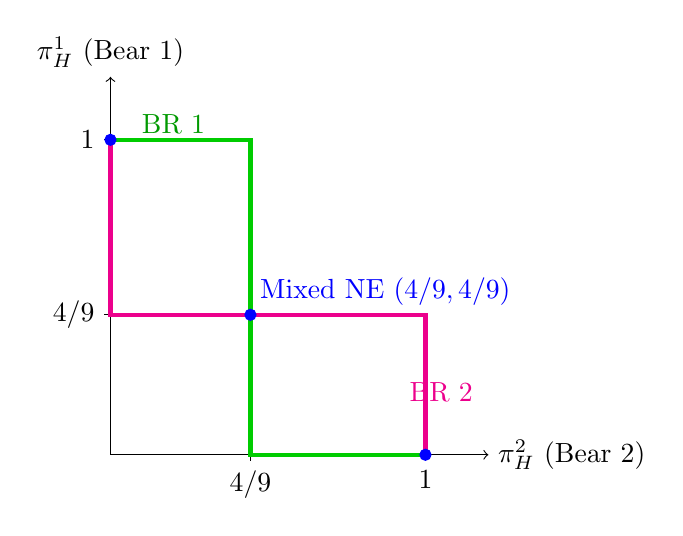
\begin{tikzpicture}[scale=4]
    % Axes
    \draw[->] (0,0) -- (1.2,0) node[right] {$\pi_H^2$ (Bear 2)};
    \draw[->] (0,0) -- (0,1.2) node[above] {$\pi_H^1$ (Bear 1)};
    
    % Ticks
    \draw (4/9, 0.02) -- (4/9, -0.02) node[below] {$4/9$};
    \draw (0.02, 4/9) -- (-0.02, 4/9) node[left] {$4/9$};
    \draw (1, 0.02) -- (1, -0.02) node[below] {$1$};
    \draw (0.02, 1) -- (-0.02, 1) node[left] {$1$};
    
    % Bear 1 Best Response (Green in slides) - Reaction to Bear 2 (x-axis)
    % If Bear 2 < 4/9, Bear 1 plays 1 (Hawk). If Bear 2 > 4/9, Bear 1 plays 0 (Dove).
    \draw[green!80!black, ultra thick] (0,1) -- (4/9,1) -- (4/9,0) -- (1,0);
    \node[green!60!black] at (0.2, 1.05) {BR 1};

    % Bear 2 Best Response (Pink in slides) - Reaction to Bear 1 (y-axis)
    % If Bear 1 < 4/9, Bear 2 plays 1 (Hawk). If Bear 1 > 4/9, Bear 2 plays 0 (Dove).
    \draw[magenta, ultra thick] (1,0) -- (1,4/9) -- (0,4/9) -- (0,1);
    \node[magenta] at (1.05, 0.2) {BR 2};
    
    % Intersections (Nash Equilibria)
    \filldraw[blue] (0,1) circle (0.5pt); % (D,H)
    \filldraw[blue] (1,0) circle (0.5pt); % (H,D)
    \filldraw[blue] (4/9,4/9) circle (0.5pt); % Mixed
    
    \node[above right, blue] at (4/9,4/9) {Mixed NE $(4/9, 4/9)$};
\end{tikzpicture}
\end{center}

\begin{remark}
There are three Nash equilibria in the Hawk-Dove game:
\begin{enumerate}
    \item Pure: Bear 1 is Hawk, Bear 2 is Dove.
    \item Pure: Bear 1 is Dove, Bear 2 is Hawk.
    \item Mixed: Each plays Hawk with probability $4/9$.
\end{enumerate}
\end{remark}

\section{Conclusion: Nash Existence Theorem}

We conclude with a fundamental theorem in Game Theory:
\begin{tcolorbox}[colback=blue!5!white,colframe=blue!75!black,title=Nash Existence Theorem]
    A game with a finite number of players, each with a finite number of pure strategies, has \textbf{at least one Nash equilibrium}.
\end{tcolorbox}
This implies that if a game has no pure strategy Nash equilibrium, it \textbf{must} have at least one mixed strategy Nash equilibrium.
